\documentclass[conference]{IEEEtran}
\IEEEoverridecommandlockouts
% The preceding line is only needed to identify funding in the first footnote. If that is unneeded, please comment it out.
\makeatletter
\def\ps@headings{
    \def\@oddhead{\hfill\thepage\hfill}
    \def\@evenhead{\hfill\thepage\hfill}
    \def\@oddfoot{}
    \def\@evenfoot{}
}
\makeatother
\pagestyle{headings}
\usepackage{cite}
\usepackage{float}
\usepackage{url}
\usepackage{amsmath,amssymb,amsfonts}
\usepackage{algorithmic}
\usepackage{graphicx}
\usepackage{textcomp}
\usepackage{xcolor}
\def\BibTeX{{\rm B\kern-.05em{\sc i\kern-.025em b}\kern-.12em
    T\kern-.1667em\lower.7ex\hbox{E}\kern-.10emX}}
\begin{document}

\title{Simulating Earthquake Stress on a Fault Line Grid using C Programming\\

\author{Brandon Proano \\ University of Central Florida \\ Email: brandon.proano@ucf.edu}

{\footnotesize \textsuperscript{}}
\thanks{}
}



\maketitle

\begin{abstract}
This paper presents my Earthquake Simulator program, written in C, that will be used by the residents of Kimbus Planet in order for them to predict earthquakes. The simulation allows the users to create their fault
lines and it displays the accumulation of stress on the planet's surface. Earthquakes are triggered when the stress at a specific point exceeds 200. This project combines algorithmic logic with terminal visualization, offering insights on to how stress accumulates on regions with and without fault lines. 
\end{abstract}


\section{Introduction}
Earthquakes are among some of the most powerful natural phenomena, presents across celestial bodies, including planet Earth and planet Kimbus.
Earthquakes have been bringing chaos and havoc to the residents of Kimbus. It is for this reason that I set out to create a program to help pinpoint Earthquakes to help predict them, in an attempt to save lives and keep the residents of planet Kimbus safe. Understanding the origins of earthquakes provides significant practical and scientific knowledge and can be extremely helpful. My interactive tool, written in C, gives the freedom to the residents to create their fault lines, display them, and simulate the accumulation of stress across the surface of their planet. 


\section{Related Work}
While other earthquake simulators exist, such as USGS ShakeMap, my approach differs from the other software options because it breaks the process down and makes it very simple and easy for a resident of planet Kimbus to use without any training or experience. Other simulators, such as USGS ShakeMap, can often be far too complex and require a great deal of training and experience. This is why my software is superior in some circumstances. 

\section{Summary}
This project is a terminal-based earthquake simulation tool written in C, designed to model the accumulation of tectonic stress across a two-dimensional grid. The simulation environment mimics the earthquake-prone surface of planet Kimbus's crust where stress accumulates over time, particularly along user-defined fault lines. These fault lines can be drawn as vertical, horizontal, diagonal, or circular shapes, each contributing uniquely to stress distribution patterns.

The simulation begins with a clean 20×20 grid that is initialized with 0's, where users interactively create, by inputting values, define fault line locations. The stress levels for each point on the grid are also initialized to zero. As the simulation progresses, points on fault lines experience more stress due to tectonic activity, whereas non-fault points accumulate less stress. When any spot on the surface of planet Kimbus reach or exceed a predefined stress level, for example, 200, an earthquake is triggered and occurs at that spot. Furthermore, the earthquake visually indicated through an ANSI color-coded terminal output. Green, yellow, and red colors represent low, medium, and high stress respectively, while earthquake points are highlighted with a red text and yellow background.

Key implementation features:
\begin{itemize}
    \item User-driven fault line creation, supporting multiple patterns including lines and circles.
    \item Dynamic stress calculation logic, using randomized stress updates that simulate realistic activity.
    \item Real-time visualization using ANSI escape codes to represent the user created fault lines as well as the stress levels. 
    \item Edge case handling for grid boundaries, ensuring fault lines and circles are rendered within the grid and don't exceed it. 
    \item Modular code design, leveraging structs and multi-dimensional arrays for organized data management.
\end{itemize}

This simulation not only strengthens understanding of earthquakes as a natural phenomenon but it also helps in better understanding and comprehending system programming, user interaction, graphical terminal display, and simulation design. It lays a foundation for building more complex simulations or even perhaps using real-world geological data in the future.

\section{System Design and Workflow}
The program consists of the following stages:
\begin{itemize}
    \item \textbf{Grid Initialization:} All stress values are initialized to zero.
    \item \textbf{Fault Line Creation:} The user can draw vertical, horizontal, diagonal, or circular fault lines.
    \item \textbf{Stress Simulation:} Each cell updates based on its status (fault/non-fault).
    \item \textbf{Visualization:} Colors represent stress levels: green (low), yellow (medium), red (high), and red-on-yellow for earthquakes.
\end{itemize}

\begin{figure}[H]
    \centering
    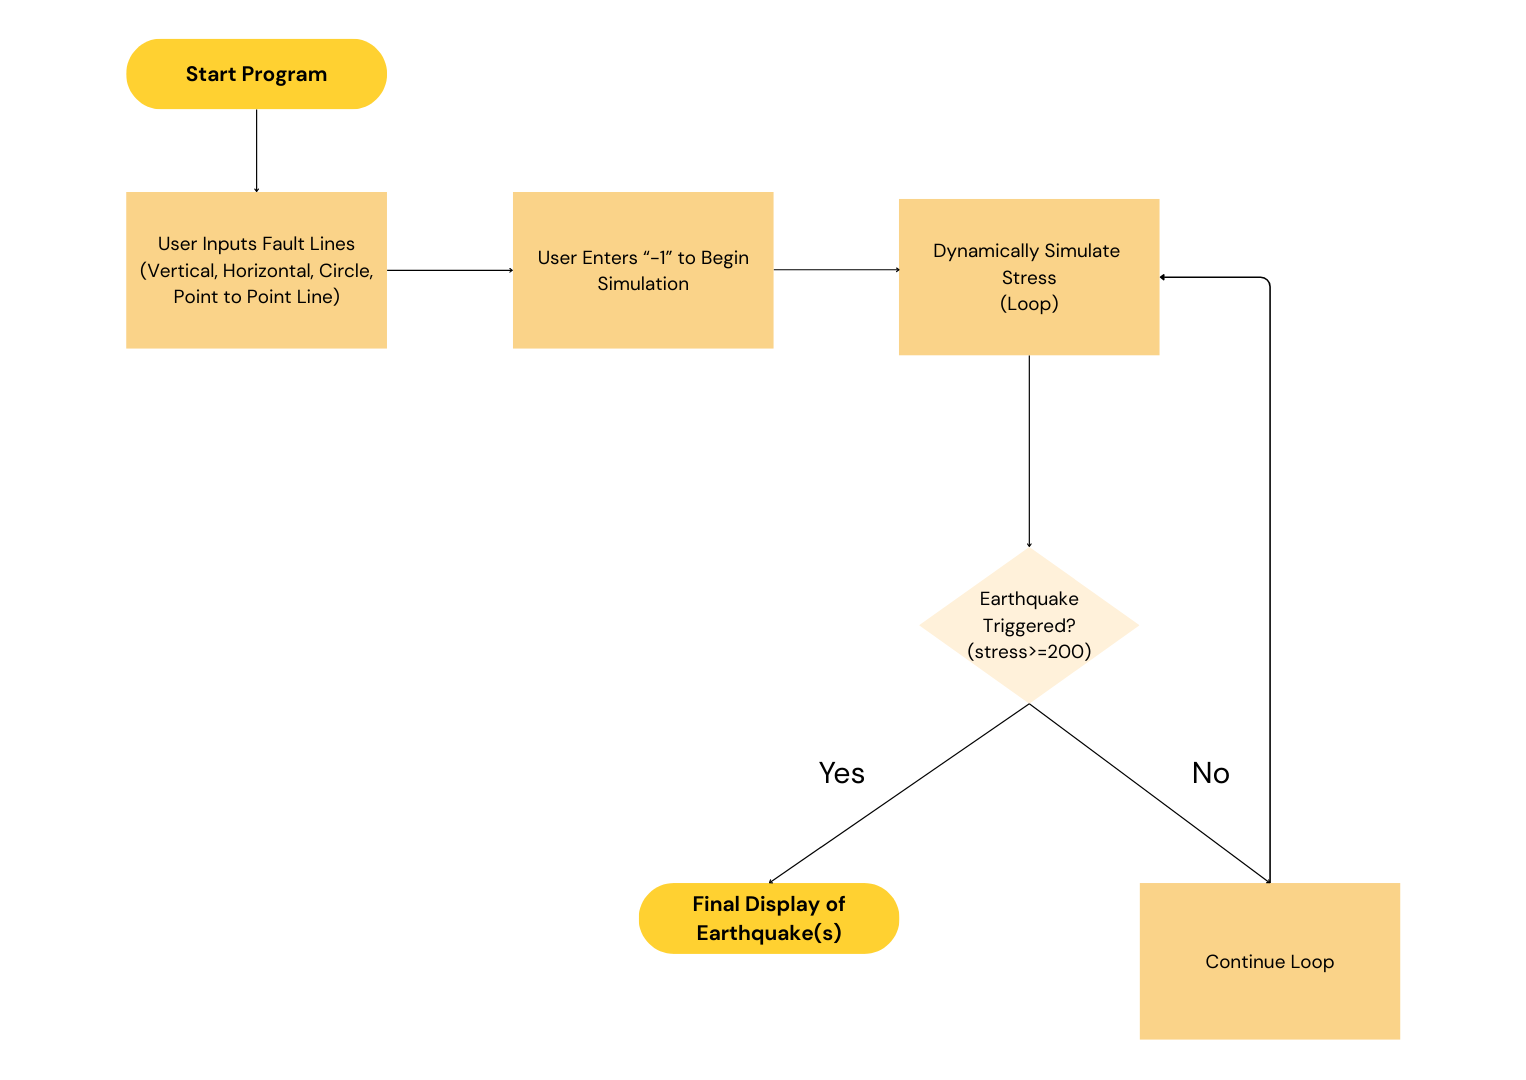
\includegraphics[width=0.9\linewidth]{workflow_diagram.png}
    \caption{Workflow diagram representing the steps of the program.}
    \label{fig:faultlines}
\end{figure}

\section{Key Takeaways}

\subsection{Understanding of Simulation Logic}

Through this project, I was able to enhance my knowledge and understanding of how simulation software and logic works. This knowledge is imperative to understand real-world phenomena, in this case, earthquakes. To be specific, I learned how to model and create dynamic systems, that require constant updating, using iterative updates (for-loops) and conditional checking. Implementing this logic gave me a deeper understanding of how might people create software to simulate other extreme phenomena, such as rogue waves and hurricanes. This foundational knowledge and experience will be invaluable to me as I continue to grow my career, pursuing projects in AI and Cybersecurity. 

\subsection{Mastery of Multidimensional Arrays and Structs in C}
This project significantly tested and strengthened my ability to work with two-dimensional arrays as well as the struct data type in C. For this project, I was able to use a struct data type, called SimulationData, in my code that held both of the two-dimensional arrays, one that represented the fault lines, and one that represented the stress across the surface. By using the struct data type along with the two-dimensional arrays, I was able to keep my code clean and modular, allowing me to easily add more arrays if needed or to access the data throughout the program without problems. This deepened my understanding low-level software, modularity, data organization, and array indexing. These are foundational skills and techniques that are widely used and applicable in both academic research and industry applications.



\subsection{Integration of User Input and Dynamic Display}\label{AA}
This project was an excellent opportunity to expand my skills when working with the command line interface. Learning how to build an extensive and interactive terminal-based application that was reading user data in real-time as well as dynamically updating the display by clearing the terminal and reprinting data gave me valuable experience. Furthermore, not only did I handle user data, dynamic updates, and terminal limitations, but I also was able to use ANSI escape codes to implement color-coded outputs which really aided in bringing this project to life. Using color codes to draw the fault lines and to display the changes in stress was excellent visual feedback and it significantly improved the usability and ease-of-use of the simulation. This skill is incredibly valuable when working with and creating all responsive terminal-based applications that rely on data visualization. 

\begin{figure}[H]
    \centering
    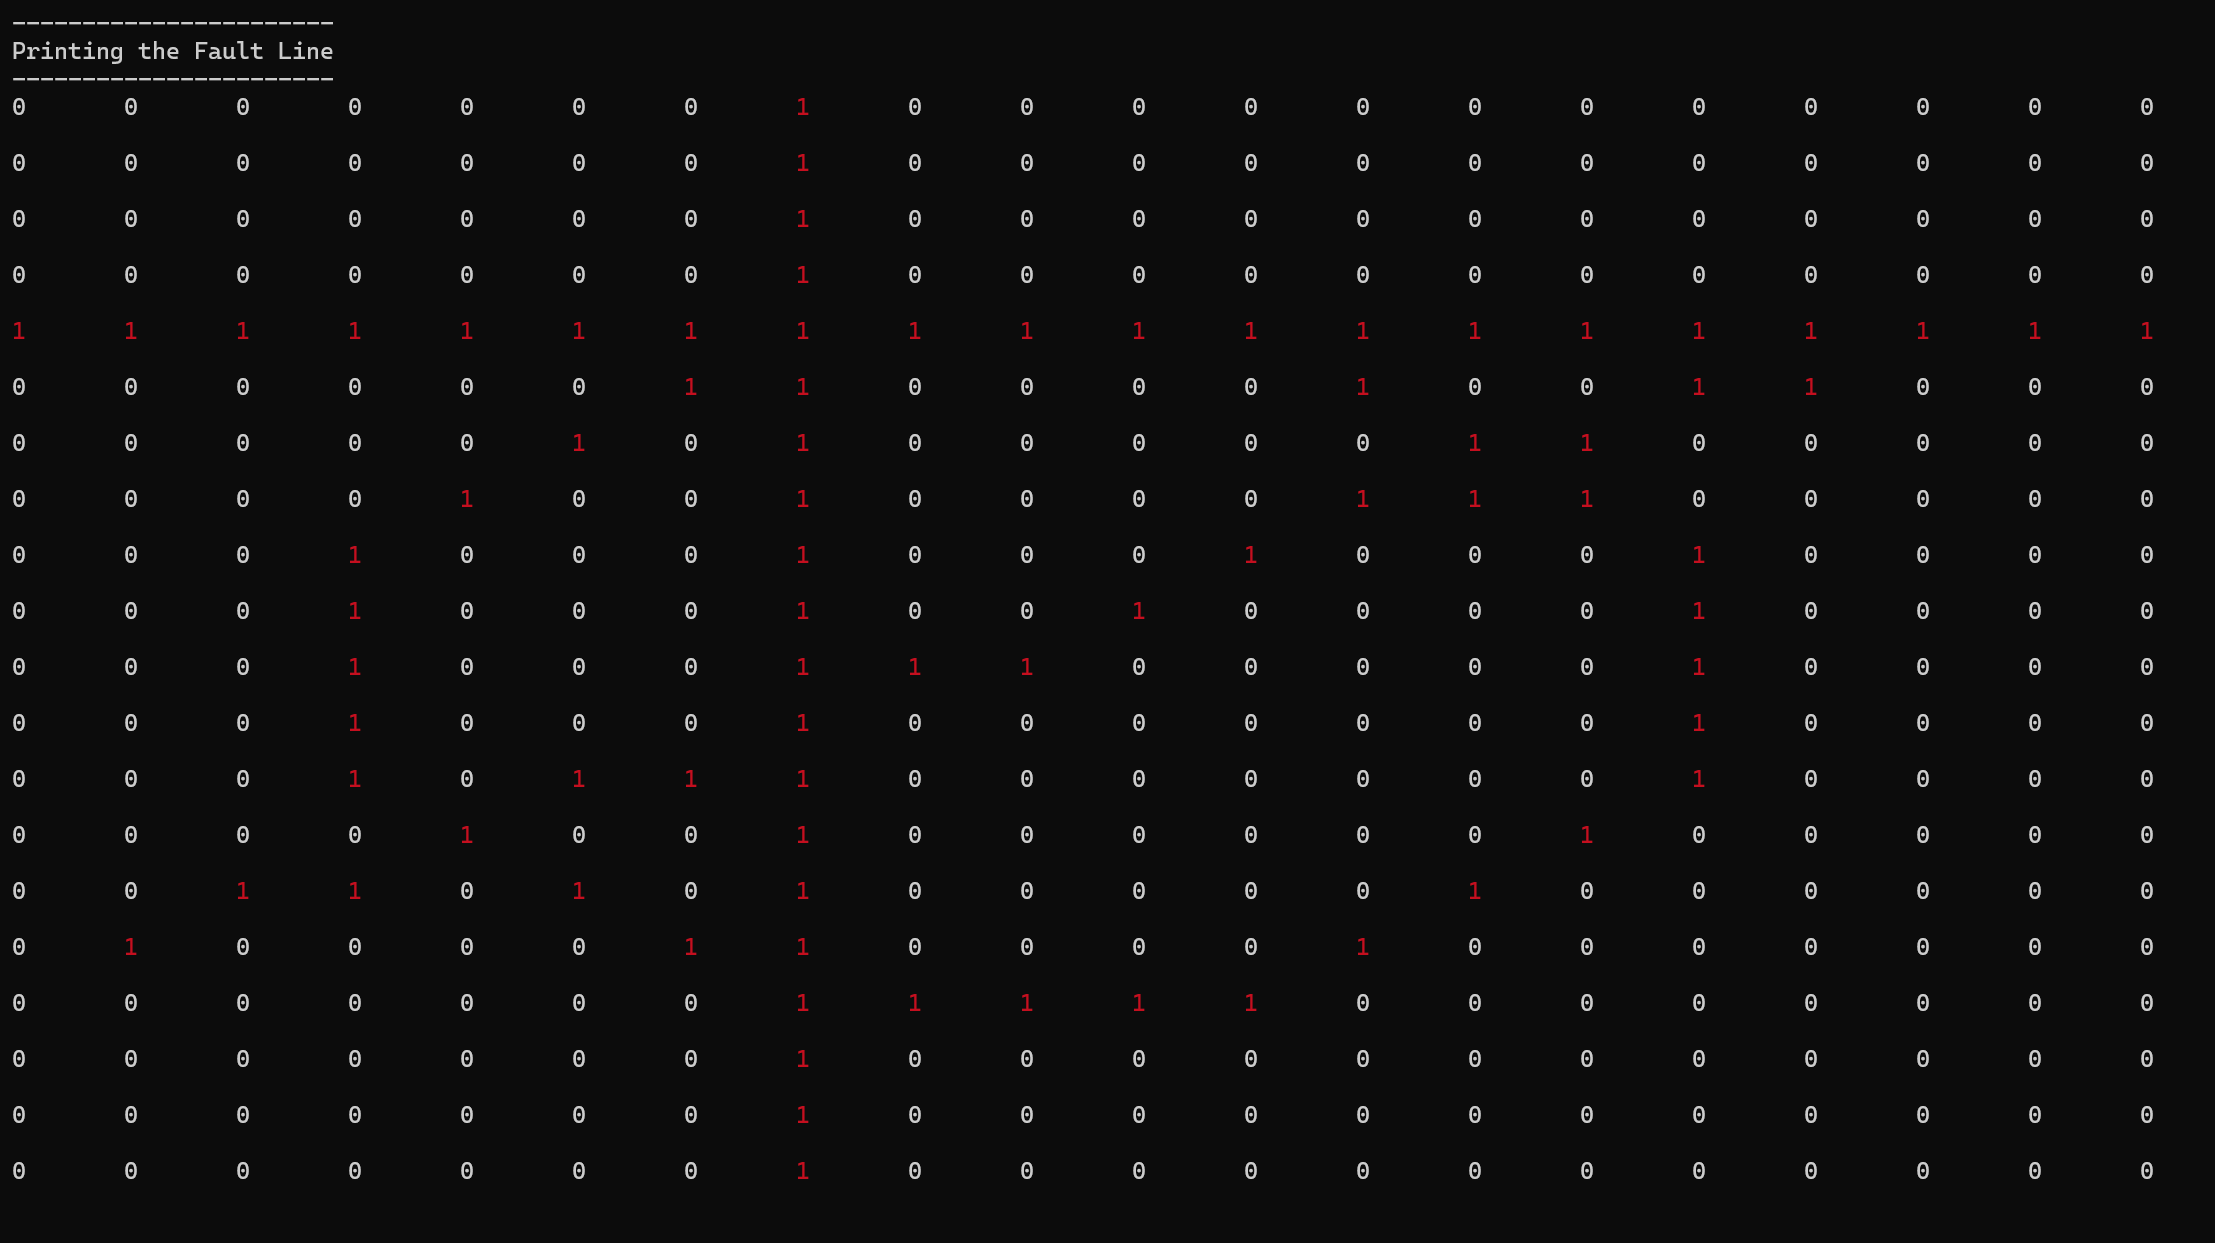
\includegraphics[width=0.9\linewidth]{fault_line_example.png}
    \caption{Visualization of the simulated fault lines with color-coded output.}
    \label{fig:faultlines}
\end{figure}

\subsection{Debugging and Edge Case Handling}
This project reinforced how important it is to debug code and handle edge cases and unexpected input. An example of this that was used in my code was preventing negative stress values as well as ensuring the visual alignment of the dynamically printed output. Edge case handling was also done with creating each individual fault line. For example, I had to validate the user input, ensuring that it was in the proper range. Furthermore, for the circle fault line, I had to ensure that the circle points were in the range, and if they were not, they would not be added to the array of fault lines. Through repeated testing and debugging, I now have valuable experience in writing bug-free and resilient code that behaves predictably under a range of user input conditions and variations. 

\begin{figure}[!htbp]
    \centering
    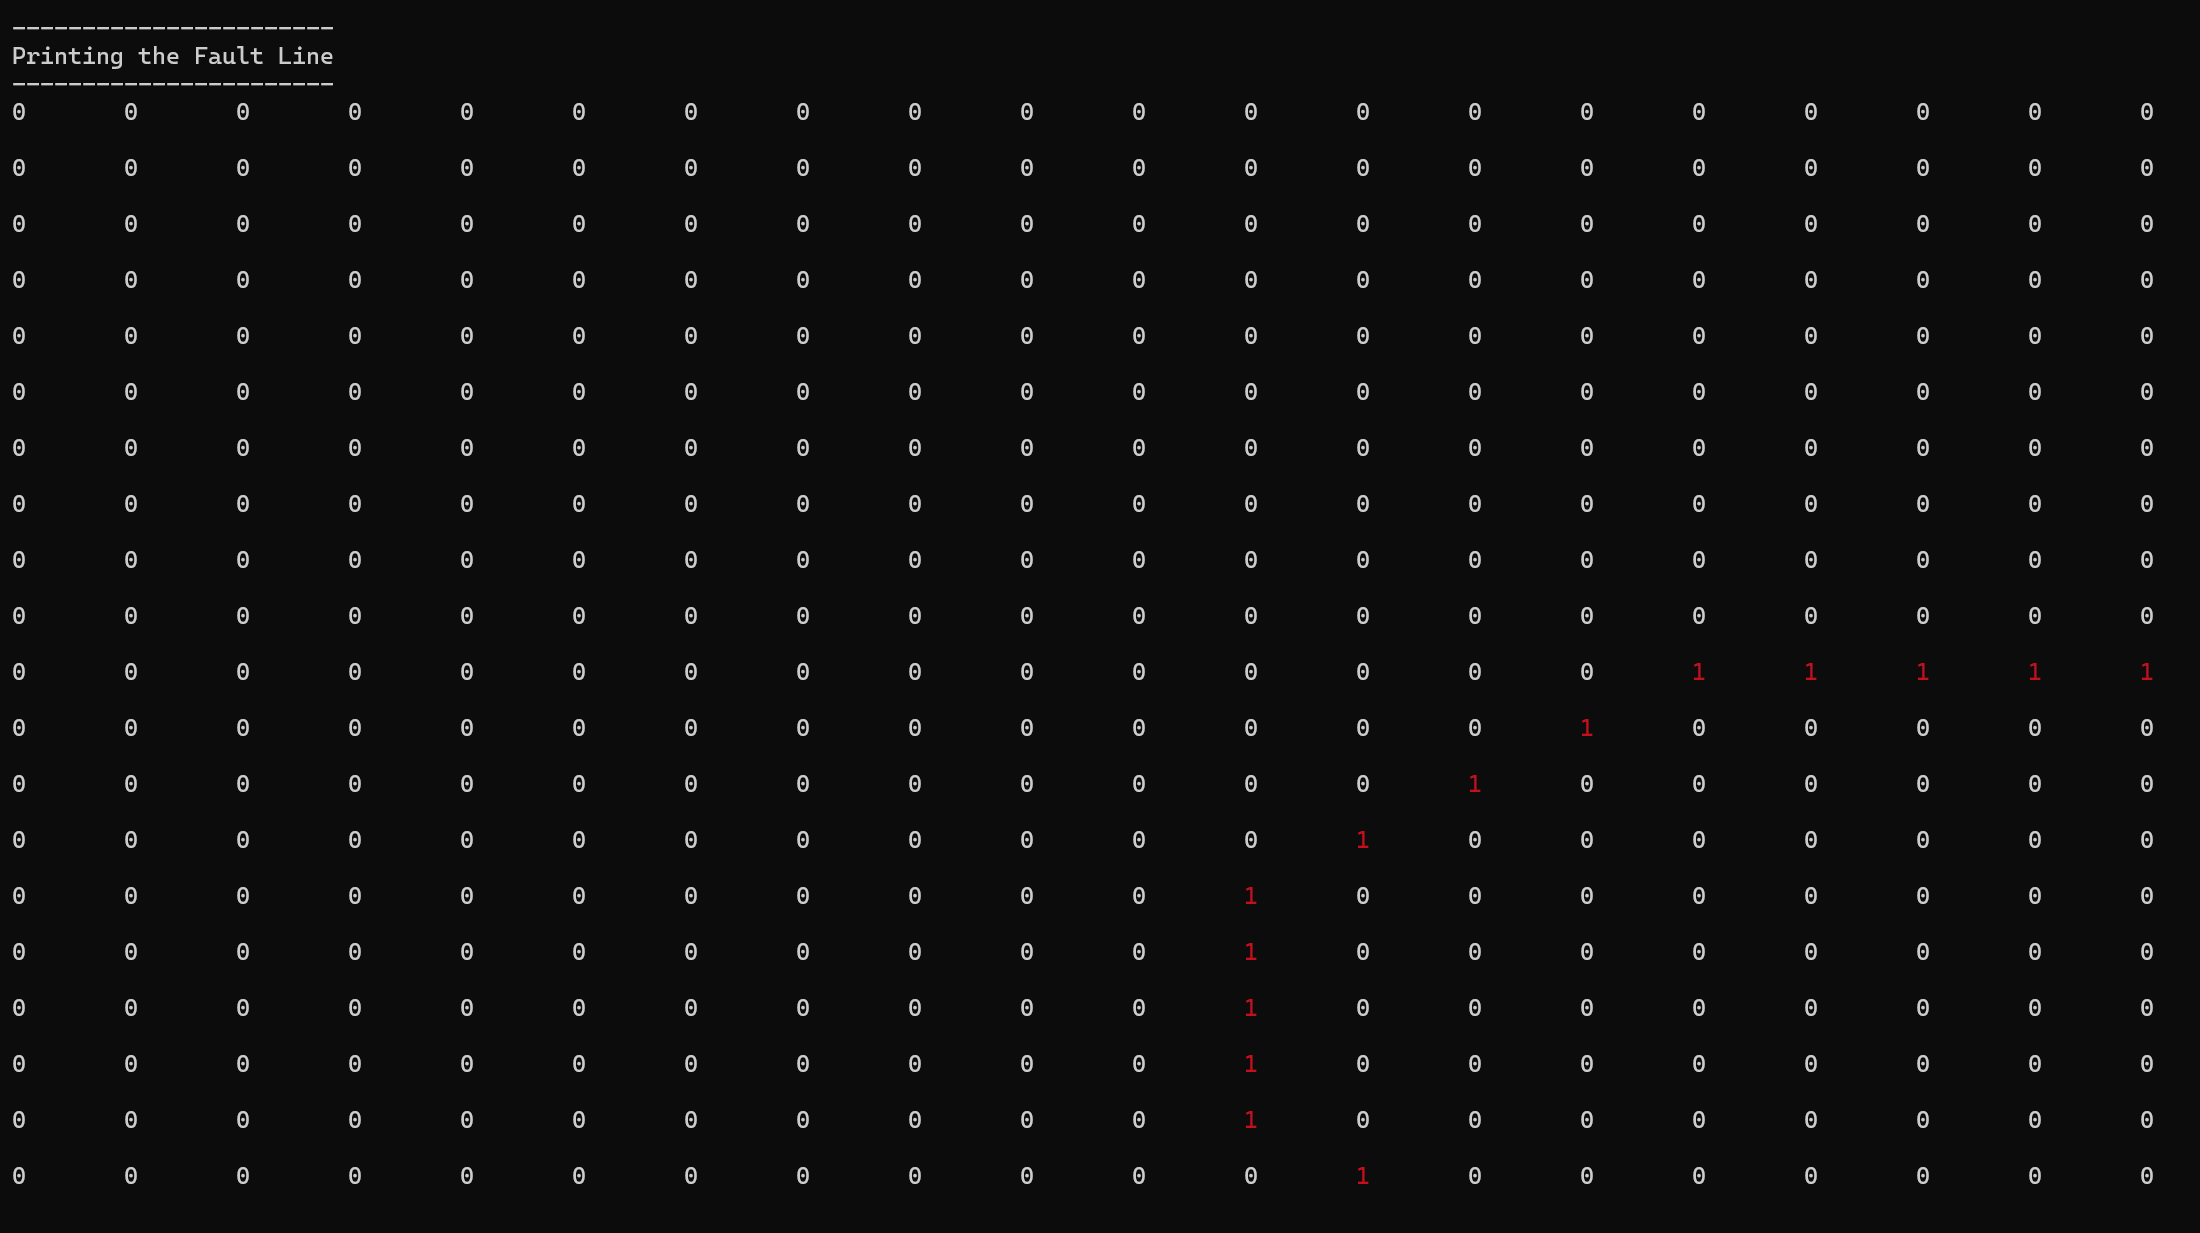
\includegraphics[width=0.9\linewidth]{cutoff_circle.png}
    \caption{A circular fault line placed near the array boundary. This tests edge case handling where portions of the shape extend beyond simulation limits.}
    \label{fig:cutoffcircle}
\end{figure}

\newpage

\section{Conclusion}
In summary, this project was a successful implementation of a simulation of tectonic stresses and earthquakes on the planet Kimbus. Having the opportunity to create this project offered me a hands-on understanding of terminal-based applications, algorithm design, and real-time user interaction. Using various tools and C programming concepts, such as multidimensional arrays, structs, and random number generation, allowed me to achieve my goal of properly simulating the fault lines and stress buildup. 

This program demonstrates the importance of visualizing and simulating real-world phenomena and natural disasters using computational models. In order to make my program more visually appealing, I used ANSI color codes that were applied on the fault lines as well as the different stress levels. Furthermore, when an earthquake or earthquakes occur, it is highlighted with a yellow background, further enhancing  the user experience for my program.

The interactive nature of the program allows the user to easily draw their own fault lines and start the simulation by simply passing specific values to the program that are neatly displayed on a prompt. Giving the user the freedom and flexibility to create the own fault lines creates a very productive learning experience for the user as they get to experiment and visually see how their changes contribute to the change in location of earthquakes. Additionally, the implementation and careful consideration of edge case behavior and handling, such as circle boundaries and stress levels, further reinforced the easy of use and robustness of the program. 

In conclusion, this project did not only deepen my understanding of C programming and technical skills, but it also improved my critical-thinking skills in system design and simulation. The experience that I have gained from debugging and optimizing the simulation has contributed to my overall growth as a programmer and student.

\newpage

\begin{thebibliography}{1}

\bibitem{bari}
A. Bari, “Bresenham's Circle Drawing Algorithm - Computer Graphics.” \textit{YouTube}. [Online]. Available: \url{https://www.youtube.com/watch?v=rOocMVYI6Zs&t=2s&ab_channel=AbdulBari}

\bibitem{ansi}
ANSI Escape Code. \textit{Wikipedia}. [Online]. Available: \url{https://en.wikipedia.org/wiki/ANSI_escape_code}

\end{thebibliography}

\end{document}
